% Created 2025-04-29 Tue 19:34
% Intended LaTeX compiler: pdflatex
\documentclass[11pt]{article}
\usepackage[utf8]{inputenc}
\usepackage[T1]{fontenc}
\usepackage{graphicx}
\usepackage{longtable}
\usepackage{wrapfig}
\usepackage{rotating}
\usepackage[normalem]{ulem}
\usepackage{amsmath}
\usepackage{amssymb}
\usepackage{capt-of}
\usepackage{hyperref}
\usepackage{minted}
\usepackage{graphicx}
\graphicspath{ {./images/} }
\author{Hankertrix}
\date{\today}
\title{Stereochemistry Notes}
\hypersetup{
 pdfauthor={Hankertrix},
 pdftitle={Stereochemistry Notes},
 pdfkeywords={},
 pdfsubject={},
 pdfcreator={Emacs 30.1 (Org mode 9.7.11)}, 
 pdflang={English}}
\begin{document}

\maketitle
\setcounter{tocdepth}{2}
\tableofcontents \clearpage\section{Definitions}
\label{sec:org88fd562}

\subsection{Isomers}
\label{sec:org22fe0c2}
Isomers are compounds that have the same molecular formula, but different structures.
\subsection{Constitutional isomers}
\label{sec:org829af7f}
Constitutional isomers are isomers that have atoms bonded together in different orders. It consists isomers containing different functional groups, different position of functional groups, and different carbon skeletons.
\subsection{Stereoisomers}
\label{sec:org17320c1}
Stereoisomers are isomers that have all the atoms connected in the same order, but differ only in the 3D orientations of their atoms in space.
\subsection{Enantiomers}
\label{sec:org91374bd}
Enantiomers are molecules that are mirror images of each other but are non-superimposable. Enantiomers rotate the polarised light in opposite directions, but with the same degree of rotation.
\subsection{Chiral carbon (chiral centre)}
\label{sec:org080bebb}
Chiral carbons are carbon atoms in a molecule that have 4 different substituents and also have a non-superimposable mirror image.
\subsection{Optically active}
\label{sec:org872d676}
Optically active just means a substance or compound \textbf{rotates} plane-polarised light.
\subsection{Optically inactive}
\label{sec:org6ae5509}
Optically inactive just means a substance or compound \textbf{does not} rotate plane-polarised light.
\subsection{Racemic mixture}
\label{sec:orgae32fb0}
A racemic mixture is a mixture that contains an equal amount of two enantiomers, which results in the mixture being optically inactive.
\subsection{Polarimeter}
\label{sec:org33df14d}
A polarimeter is a device that measures the rotation \(\alpha\) of plane-polarised light in degrees.
\subsection{Dextrorotatory (+)}
\label{sec:org97df1df}
Dextrorotatory refers to the \textbf{clockwise} rotation of plane-polarised light. Molecules that are dextrorotatory are labelled \(R\), which is from the Latin word for "right".
\subsection{Laevorotatory (-)}
\label{sec:orga40cba1}
Laevorotatory refers to the \textbf{anti-clockwise} rotation of plane-polarised light. It is shown using the symbol \(S\) for left or \(-\). Molecules that are laevorotatory are labelled \(S\), which is from the Latin word for "left".
\subsection{Diastereomer}
\label{sec:org5640c3e}
Diastereomers are stereoisomers which are \textbf{not mirror images}. Molecules with more than one chiral centre can have diastereomers.
\subsection{Achiral molecules}
\label{sec:org76bdf76}
Achiral molecules are molecules that are \textbf{identical} to the mirror images. Achiral molecules are optically inactive.
\subsection{Meso compounds}
\label{sec:org8080b83}
Meso compounds are compounds that contain chiral carbons, but the compound as a whole is achiral. Meso compounds are optically inactive.

\newpage
\subsection{Prochirality}
\label{sec:org21a5083}
Prochirality refers to a molecule that is not chiral, but can become chiral by a single alteration. A \(sp^3\) carbon with only 2 groups that are the same is a prochirality centre.

\[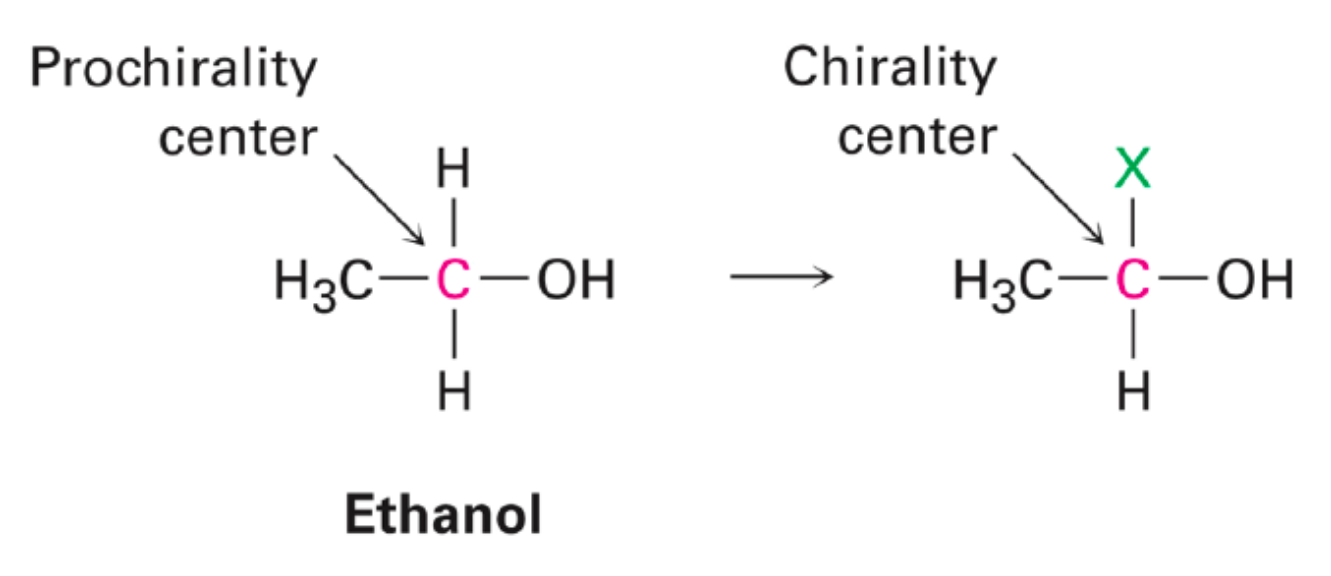
\includegraphics[width = \textwidth]{prochirality}\]
\subsection{Pro-S and Pro-R}
\label{sec:org18aaa51}

\[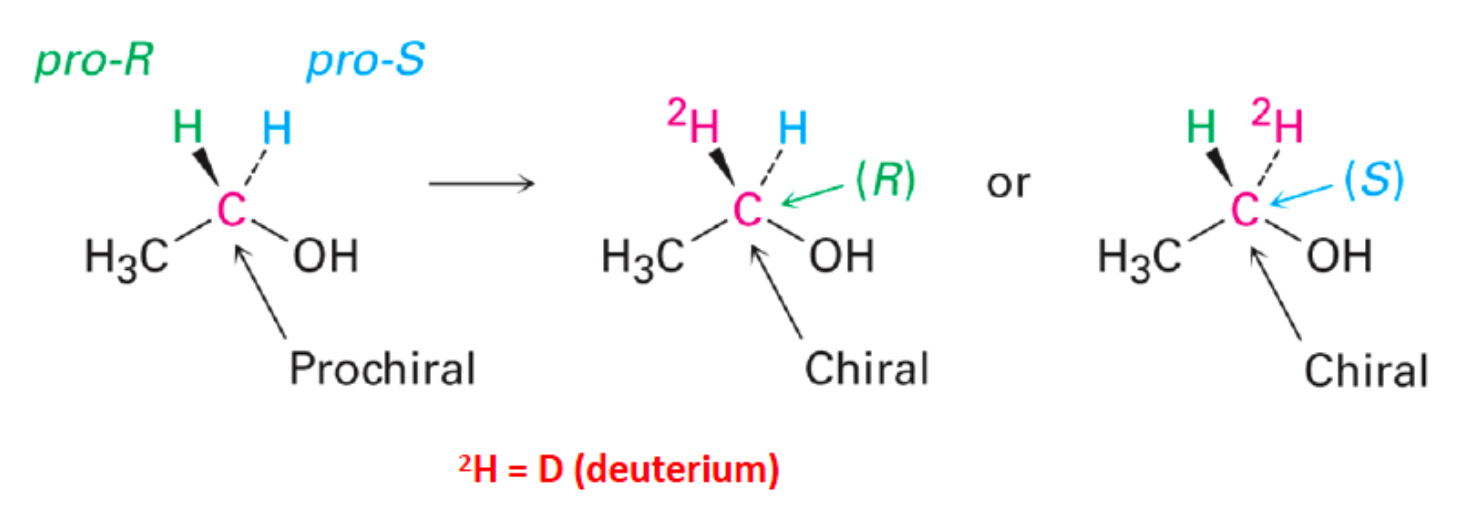
\includegraphics[width = \textwidth]{pro-s-and-pro-r}\]
\subsubsection{Pro-S}
\label{sec:org642947a}
Pro-S is a prochiral centre that will become the S configuration when an alteration is done.
\subsubsection{Pro-R}
\label{sec:org2e3cdad}
Pro-R is a prochiral centre that will become the R configuration when an alteration is done.
\subsection{Cycloalkanes}
\label{sec:org9e4cef6}
Cycloalkanes are saturated cyclic hydrocarbons and have the general formula (\(C_nH_{2n}\)).
\subsubsection{Stereoisomers}
\label{sec:org311a524}
Cycloalkanes are less flexible, so there is much less conformation freedom. Due to the cyclic structure, cycloalkanes have 2 faces when viewed edge-on, which are the "top-face" and the "bottom-face".

\[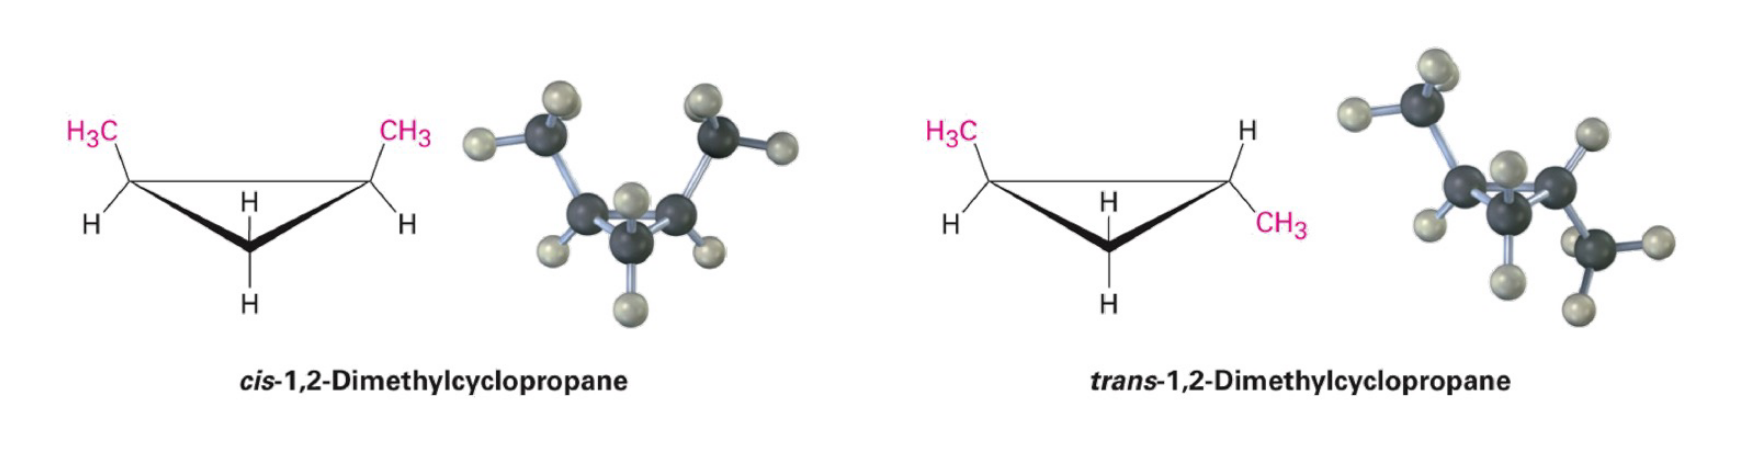
\includegraphics[width = \textwidth]{top-and-bottom-faces}\]
\subsection{Ring strain}
\label{sec:org57de9b1}

\subsubsection{Angle strain}
\label{sec:org6e30c86}
Angle strain refers to the expansion or compression of bond angles away from the most stable bond angle.
\subsubsection{Torsional strain}
\label{sec:orgc014c9e}
Torsional strain refers to the eclipsing of bonds on neighbouring atoms.
\subsubsection{Steric strain}
\label{sec:org45da7f3}
Steric strain refers to the repulsive interactions between non-bonded atoms in close proximity.
\subsection{Axial bonds}
\label{sec:org66e828d}
Axial bonds refer to the bonds that are \textbf{parallel} to the axis of symmetry of a ring.
\subsection{Equatorial bonds}
\label{sec:org240fa79}
Equatorial bonds refer to the bonds that are \textbf{perpendicular} to the axis of symmetry of a ring.

\newpage
\section{Determining chirality}
\label{sec:org59425da}
\begin{enumerate}
\item Look at the four atoms directly attached to the chiral carbon, and rank them according to the sequence rule.
\item With the lowest priority group \textbf{pointing away} (into the plane of the paper or screen), look at the remaining 3 groups in a plane.
\item \textbf{Clockwise} is designated \(R\) (from the Latin word for "right").
\item \textbf{Counterclockwise} is designated \(S\) (from the Latin word for "left").
\end{enumerate}

\[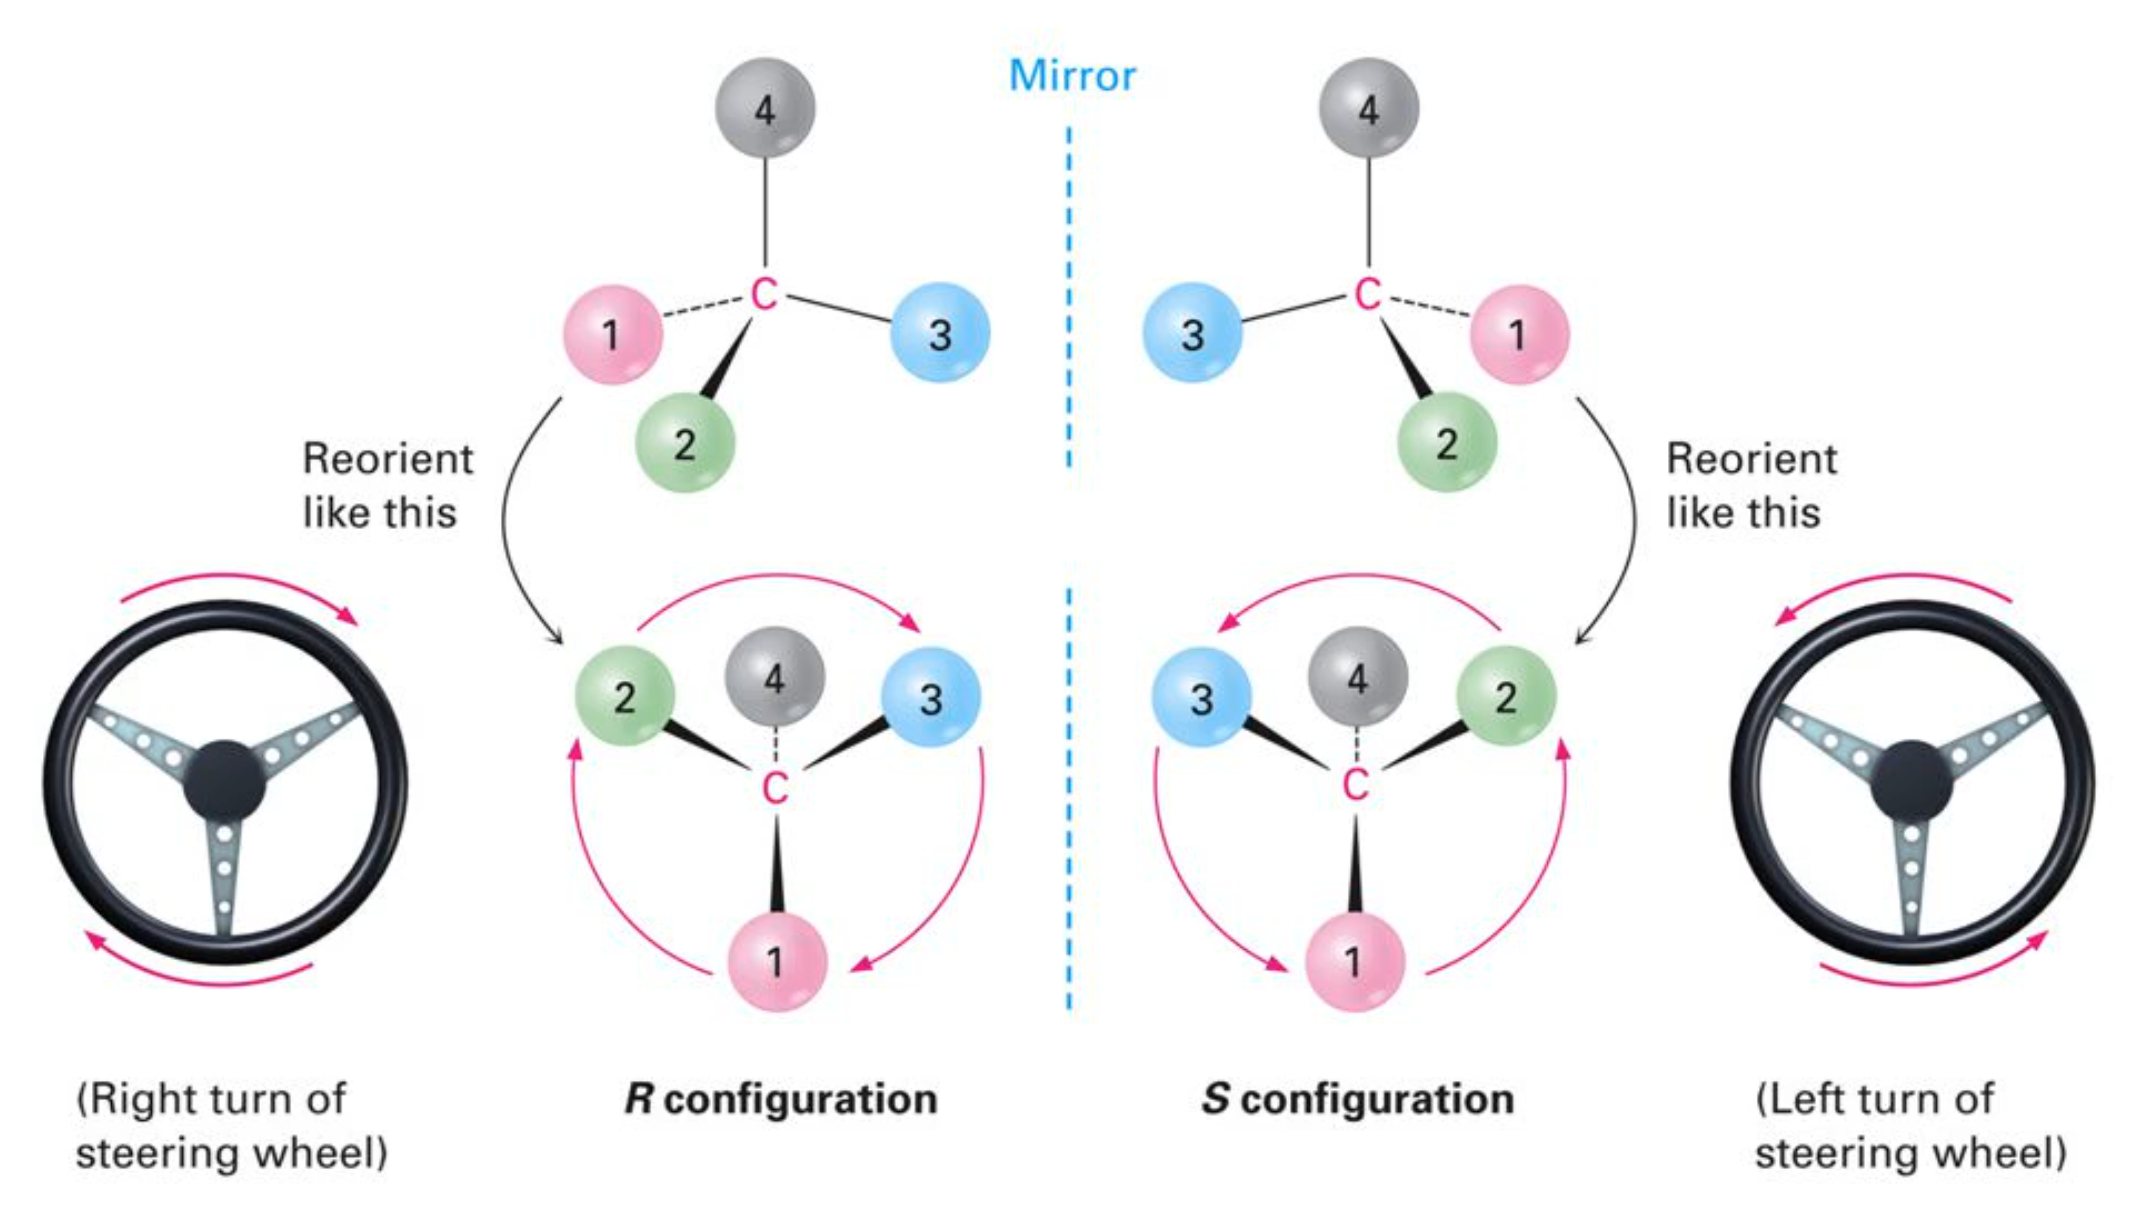
\includegraphics[width = \textwidth]{r-and-s-configuration}\]
\subsection{Important notes}
\label{sec:orgd5f3275}
\begin{itemize}
\item A \textbf{wedge} means that the group is pointing \textbf{towards} you.
\item A \textbf{dashed or dotted wedge} means the group is pointed \textbf{away} from you.
\item If the \textbf{lowest priority group} is pointed \textbf{towards} you, you can still proceed as normal, but remember to \textbf{REVERSE} the direction that you have determined.
\end{itemize}

\newpage
\subsection{Sequence rule [Cahn-Ingold-Prelog (CIP) rule]}
\label{sec:orgfa65a46}
\begin{enumerate}
\item Compare the atomic number of the atoms directly attached to the chiral carbon. The group having the atom of the \textbf{higher atomic number} receives \textbf{higher priority} (i.e. number 1).
\item If the groups have no atoms with a higher atomic number, then the number of atoms in the group should be considered. The group with the \textbf{greater} number of atoms is given a \textbf{higher priority}. For example, the priority of a \(-C(CH_3)_3\) group will be higher than a \(-CH(CH_3)_2\) group, which itself is higher in priority than a \(-CH_2CH_3\) group.
\item If a decision cannot be reached by ranking the first atom in the substitute groups, look at the second, third, or fourth atoms until the difference is found.
\item Multiple-bonded atoms are equivalent to the same number of single-bonded atoms:
\[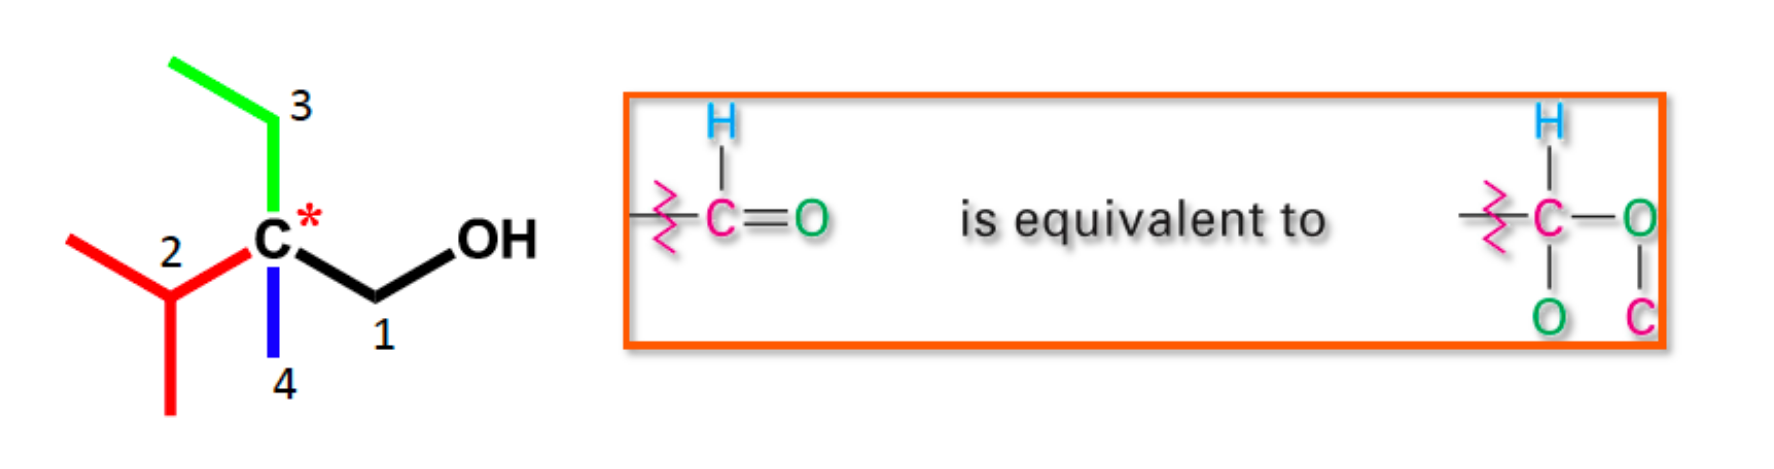
\includegraphics[width = \textwidth]{double-bond-equivalent}\]
\end{enumerate}

\newpage
\section{Examples of ring strain}
\label{sec:org1d5df58}

\subsection{Cyclopropane}
\label{sec:orgd4ddbf3}
\begin{itemize}
\item It is planar, and has a 60 degree bond angle.
\item The shape around the carbon atoms are distorted, which weakens the \(sp^3\) bond.
\item The hydrogen atoms are eclipsed.
\end{itemize}

\[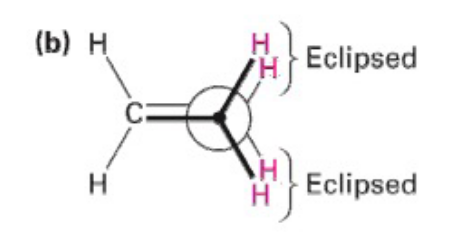
\includegraphics[scale = 0.75]{cyclopropane}\]
\subsection{Cyclobutane}
\label{sec:org5a9bb83}
\begin{itemize}
\item It has torsional and ring strain, but has less angle strain and more torsional strain than cyclopropane due to the larger number of ring hydrogens, and their proximity to each other.
\item It is slightly bent out of plane (25 degrees).
\item The bend in the ring increases angle strain but decreases torsional strain.
\end{itemize}

\[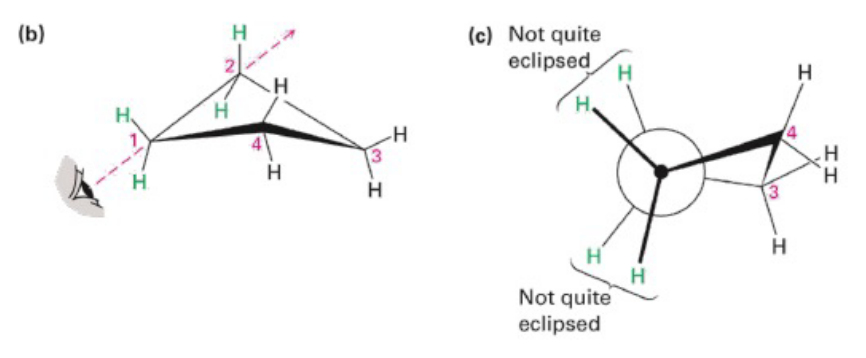
\includegraphics[scale = 0.75]{cyclobutane}\]

\newpage
\subsection{Cyclopentane}
\label{sec:org13f9459}
\begin{itemize}
\item Planar cyclopentane would have no angle strain but very high torsional strain.
\item Hence, actual conformations of cyclopentane are non-planar to reduce torsional strain.
\item There are 4 carbon atoms in a plane and the \(5^{th}\) carbon atom is above or below the plane.
\item It looks like an envelope.
\item Most of the hydrogen atoms are nearly staggered with respect to their neighbours.
\end{itemize}

\[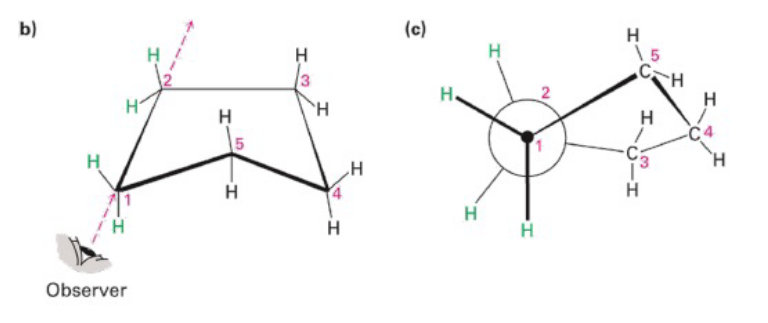
\includegraphics[scale = 0.75]{cyclopentane}\]

\newpage
\section{Conformations of cyclohexane}
\label{sec:org6abe2b0}
\begin{itemize}
\item The cyclohexane ring is free of angle strain and torsional strain.
\item The conformation has alternating atoms in a common plane and tetrahedral angles between all carbons.
\item This is called a \textbf{chair conformation}.
\item All \(C-C-C\) bond angles are near the \(109.5^{\circ}\) tetrahedral value, and all neighbouring \(C-H\) bonds are staggered.
\end{itemize}
\subsection{Drawing the chair conformation}
\label{sec:orgb2e96b0}
\begin{enumerate}
\item Draw two parallel lines, slanted downwards and slightly offset from each other. This means that 4 of the cyclohexane carbons lie in a plane.
\[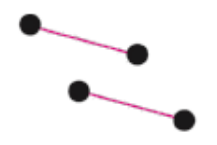
\includegraphics[scale = 0.75]{cyclohexane-drawing-step-1}\]

\item Place the topmost carbon atom above and to the right of the plane of the other 4, and connect them.
\[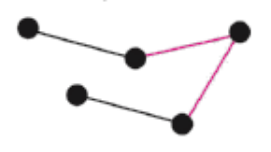
\includegraphics[scale = 0.75]{cyclohexane-drawing-step-2}\]

\item Place the bottommost carbon atom below and to the left of the plane of the middle four, and connect the bonds. Note that the bonds to the bottommost carbon atom are parallel to the bonds on the topmost carbon.
\[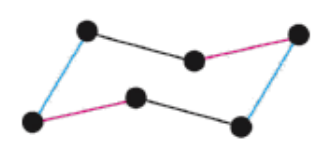
\includegraphics[scale = 0.75]{cyclohexane-drawing-step-3}\]
\end{enumerate}
\subsubsection{Alternative method}
\label{sec:orgcd7f7b6}
\[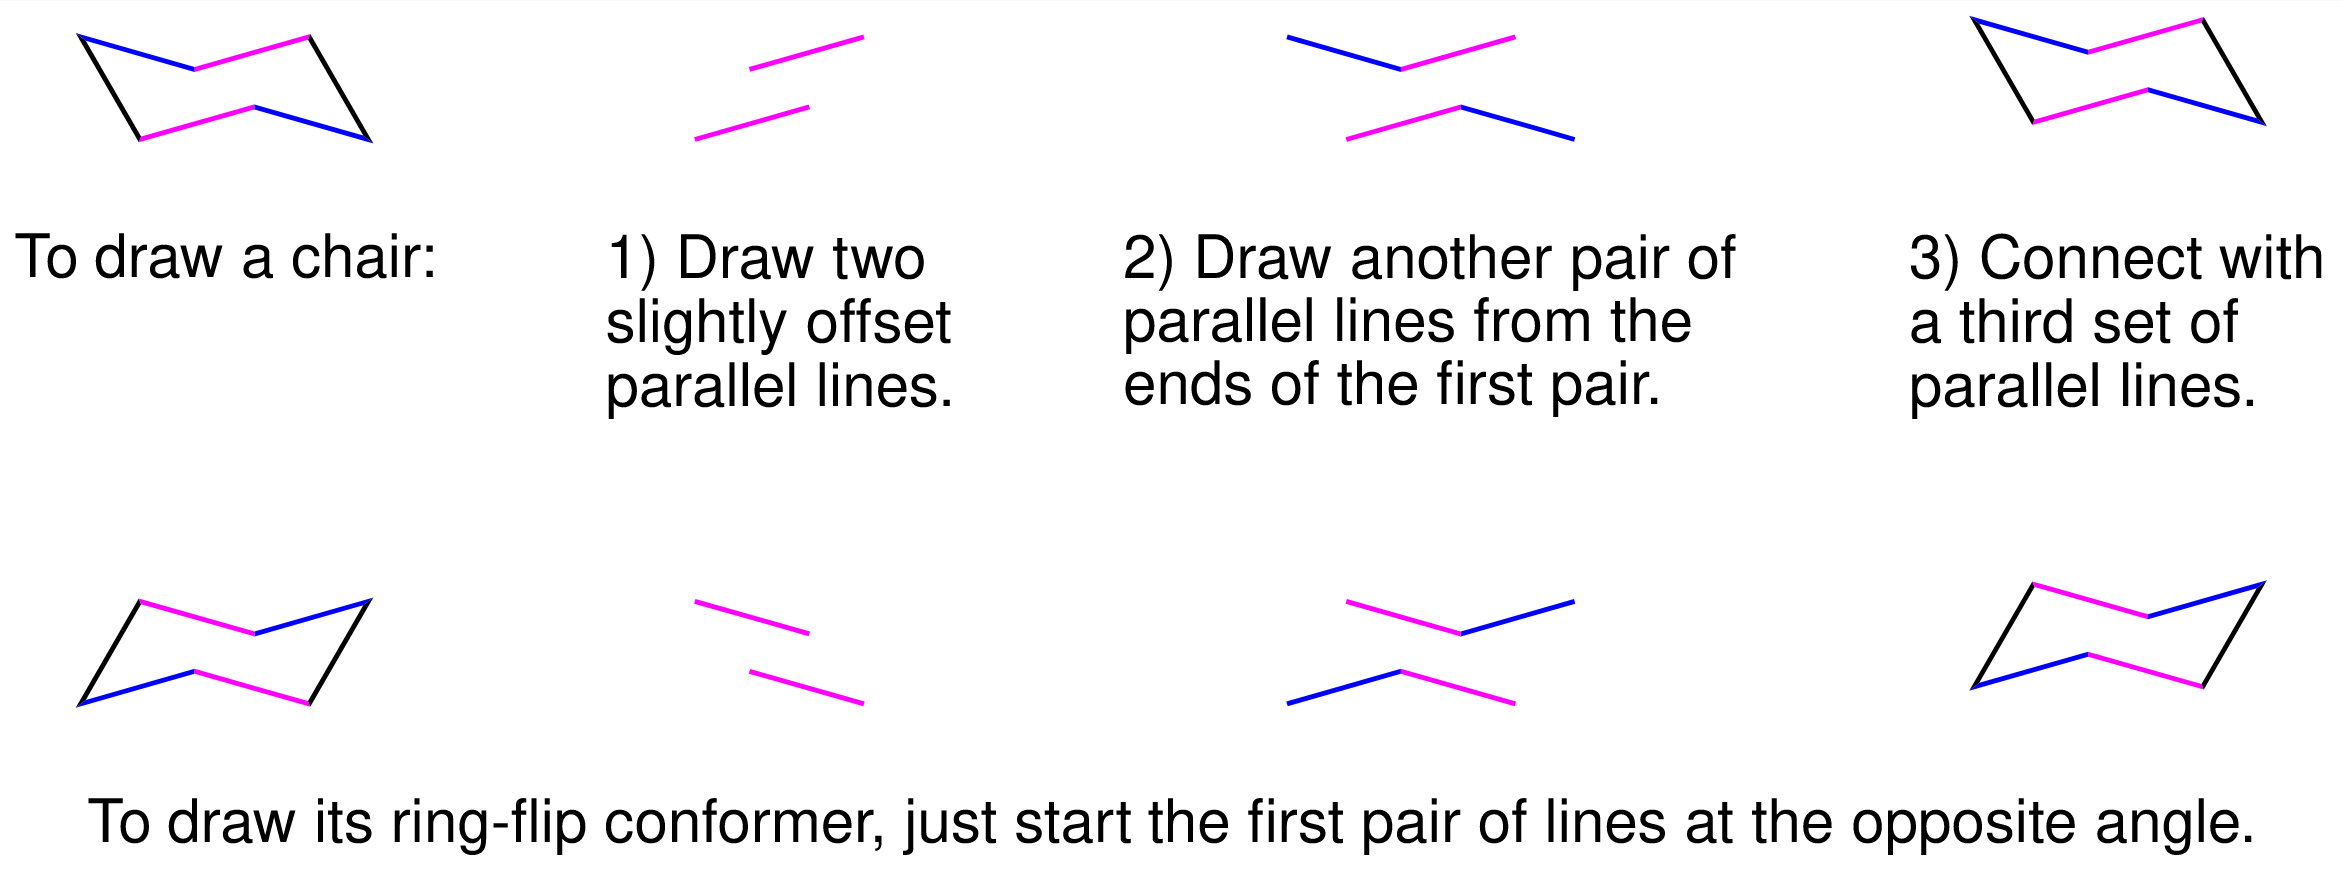
\includegraphics[width = \textwidth]{chair-conformation-steps}\]
\subsubsection{Final molecule}
\label{sec:orge47e058}
\[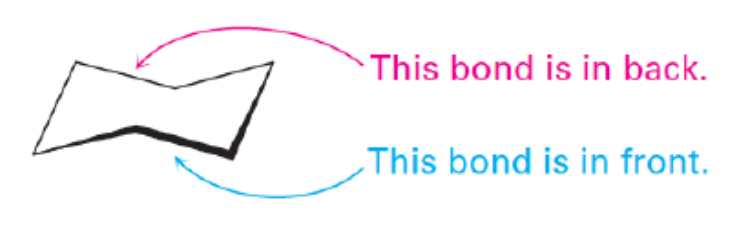
\includegraphics[scale = 0.75]{final-cyclohexane-molecule}\]
\subsection{Axial and equatorial position}
\label{sec:orga0227a0}
\[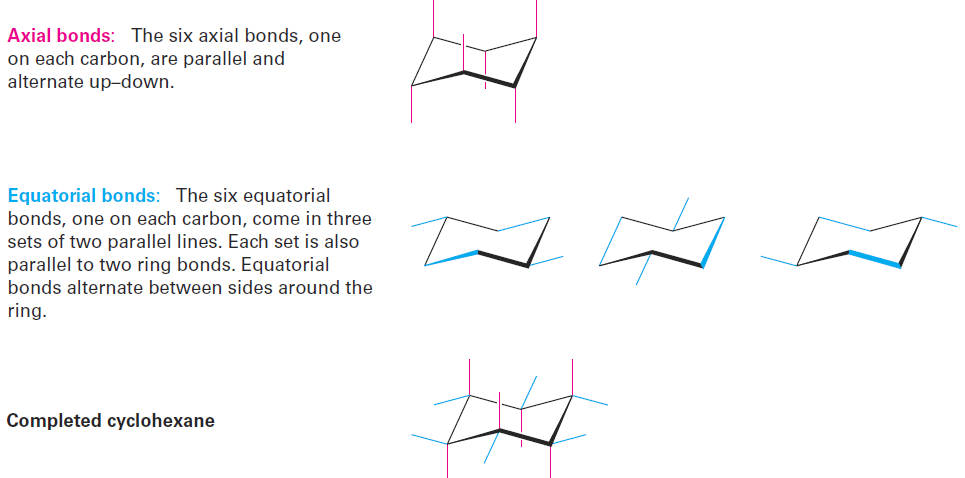
\includegraphics[width = \textwidth]{axial-and-equatorial-bonds}\]
\subsection{Ring flip}
\label{sec:org819cc17}
The chair conformations of cyclohexane readily interconvert, resulting in the exchange of axial and equatorial position by a \textbf{ring-flip}.
\[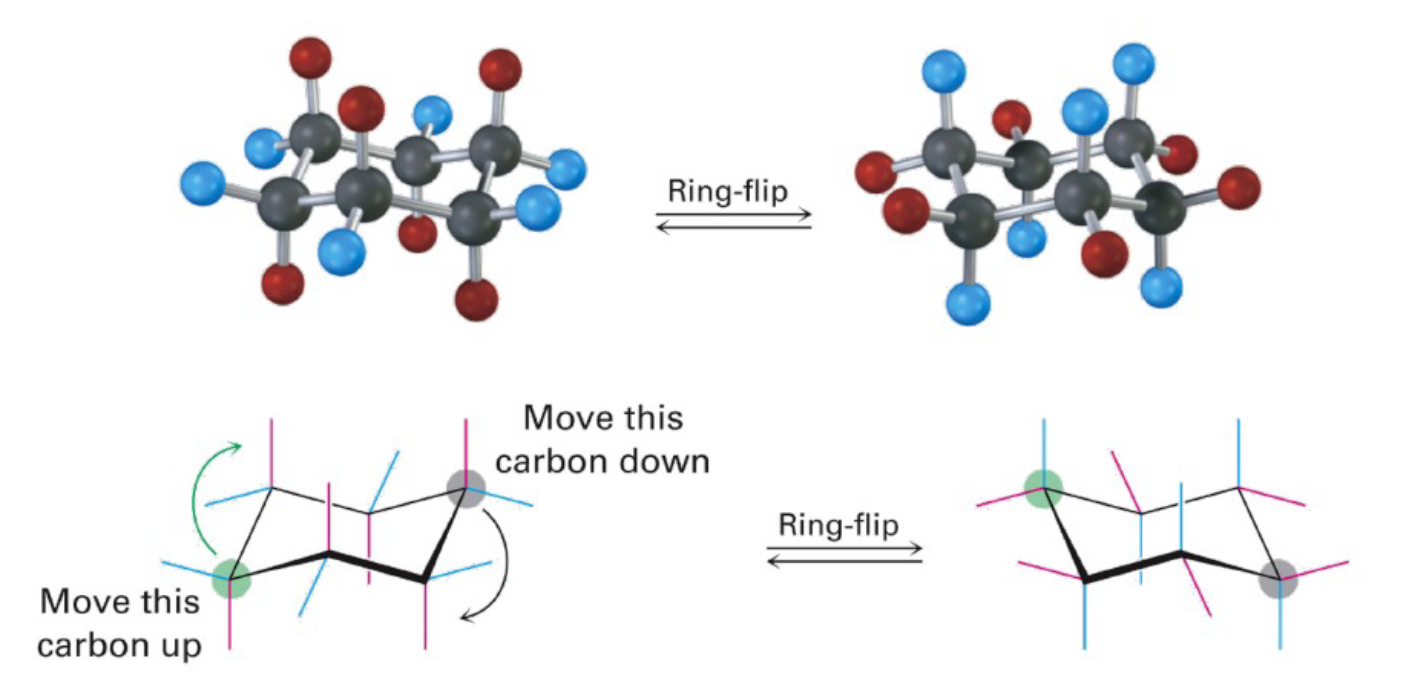
\includegraphics[width = \textwidth]{ring-flip-1}\]
\[$$\hrule$$\]
\[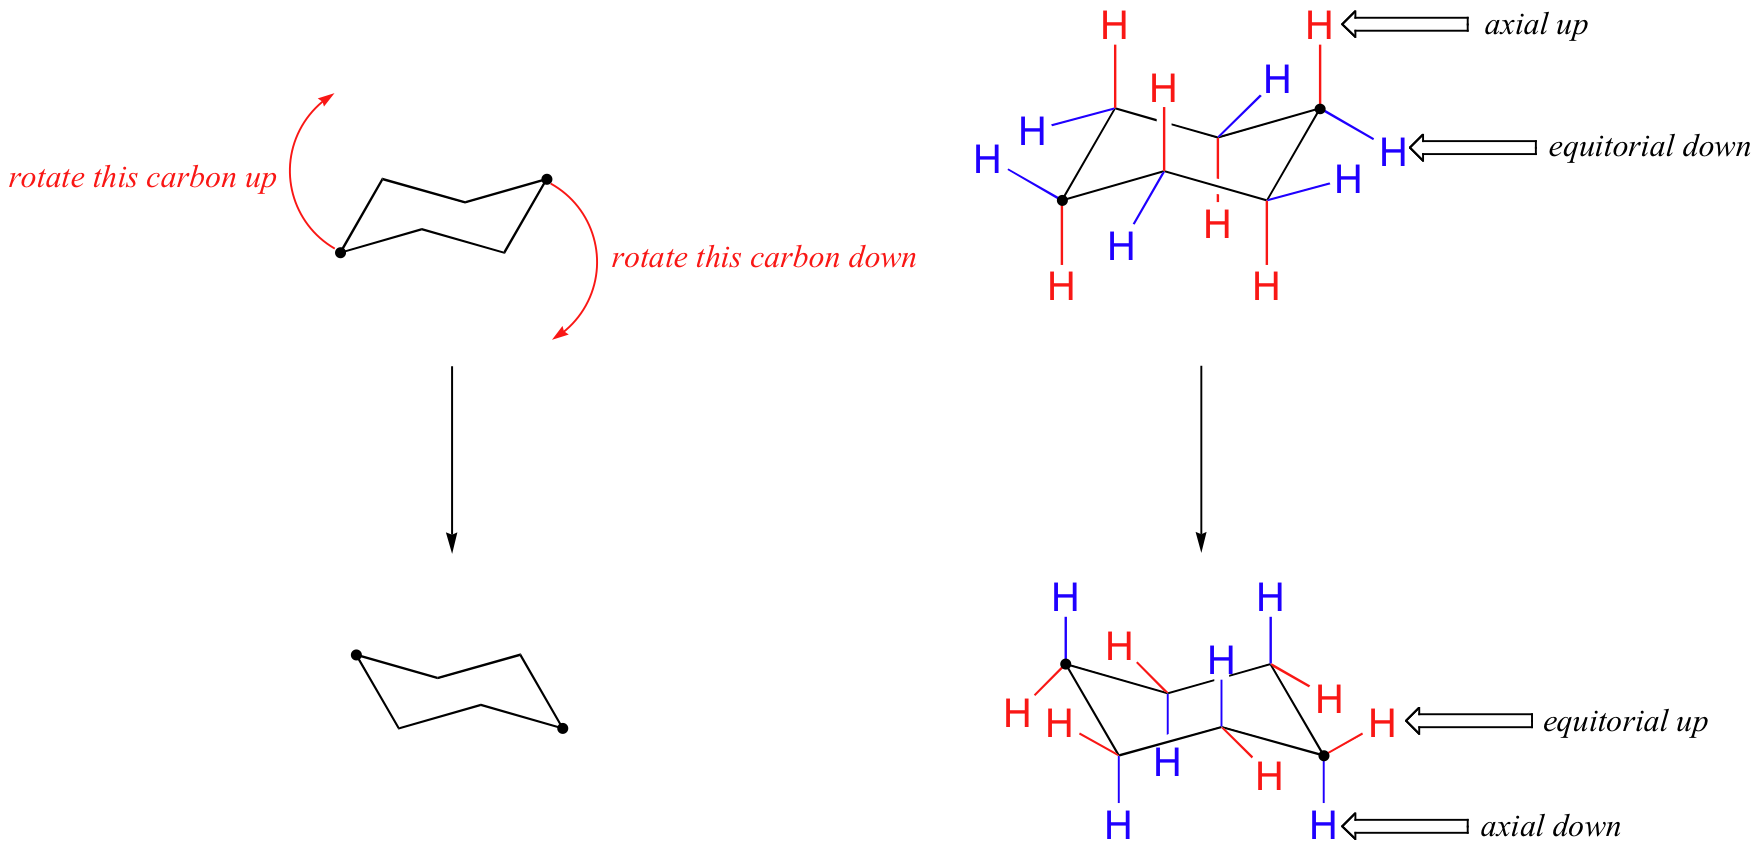
\includegraphics[width = \textwidth]{ring-flip-2}\]
\end{document}
